\documentclass{beamer}
\usepackage[utf8]{inputenc}
\usepackage{adjustbox}
\usepackage{array,ragged2e}
\usepackage{longtable}
\usepackage{pdflscape}
\usepackage{makecell}
\usepackage[font=tiny]{caption}
\usepackage{booktabs}
\usepackage[capposition=bottom]{floatrow}

\usepackage{amssymb}
\usepackage{amsfonts}
\usepackage{amsthm}
\usepackage{amsmath}
\usepackage{amsmath,systeme}
\usepackage{spalign}
\usepackage{tikz}
\usepackage{nicematrix}
\usepackage{float}
\usepackage{lmodern}
\usepackage{graphicx}
\usetikzlibrary{tikzmark}
\usetikzlibrary{arrows.meta}
\usepackage{wasysym}
\usepackage{fontawesome}

\floatstyle{plaintop}
\restylefloat{table}
\usepackage[edges]{forest}
\usepackage{subfig}

% Grey Box Hightlight
\usepackage{tcolorbox}

% Fancy table
\usepackage{tcolorbox}
\usepackage{tabularx}
\usepackage{array}
\usepackage{colortbl}
\tcbuselibrary{skins}

\newcolumntype{Y}{>{\raggedleft\arraybackslash}X}


% Code Listing Settings
\usepackage{listings}
\lstset{
	language=Python,
	basicstyle=\ttfamily,
	aboveskip={1.0\baselineskip},
	belowskip={1.0\baselineskip},
	columns=fixed,
	extendedchars=true,
	breaklines=true,
	tabsize=4,
	prebreak=\raisebox{0ex}[0ex][0ex]{\ensuremath{\hookleftarrow}},
	frame=lines,
	showtabs=false,
	showspaces=false,
	showstringspaces=false,
	keywordstyle=\color[rgb]{0.627,0.126,0.941},
	commentstyle=\color[rgb]{0.133,0.545,0.133},
	stringstyle=\color[rgb]{01,0,0},
	numbers=left,
	stepnumber=1,
	numbersep=10pt,
	captionpos=t,
	escapeinside={\%*}{*)}
}

\newcommand{\subf}[2]{%
	{\small \begin{tabular}[t]{@{}c@{}}
			\mbox{}\\[-\ht\strutbox]
			#1\\#2
	\end{tabular}}%
}

\usetheme{Madrid}
\usecolortheme{default}
\useinnertheme{circles}

\setbeamertemplate{footline}[text line]{%
	\parbox{\linewidth}{\hfill\insertpagenumber}}
\setbeamertemplate{navigation symbols}{}

\setbeamertemplate{caption}[numbered]

\definecolor{UCLAblue}{RGB}{39, 116, 174}
\definecolor{UCLAgold}{RGB}{255, 209, 0}

\setbeamercolor*{palette primary}{bg=UCLAblue, fg=UCLAgold}
\setbeamercolor*{palette secondary}{bg=white, fg=black}
\setbeamercolor*{palette tertiary}{bg=white, fg=black}
\setbeamercolor*{palette quaternary}{bg=white,fg=black}
\setbeamercolor{structure}{fg=UCLAblue} % itemize, enumerate, etc
\setbeamercolor{section in toc}{fg=UCLAblue} % TOC sections

\tcbset{tab2/.style={enhanced,fonttitle=\bfseries,fontupper=\footnotesize,
		colback=yellow!10!white,colframe=UCLAblue,colbacktitle=yellow!10!white,
		coltitle=black,center title}}
	
\def\Arrow{\raisebox{-.5\height}{\scalebox{4}{$\Rightarrow$}}}

\graphicspath{{/Users/zionsheng/Desktop/Duke/23fa/CS590/final-proj/double-descent/images}}

% \let\footnoterule\relax
\renewcommand{\footnoterule}{%
	\kern 0.1mm
	\hrule width \textwidth height 0.8pt
	\kern 1mm
}

\newtcbox{\mybox}[1][red]{on line,
	colback=#1, colframe=#1, boxsep=0pt, boxrule=0pt, size=small, arc=1mm}

\usepackage{hyperref}
\hypersetup{
	colorlinks=true,
	citecolor=blue,
	linkcolor=blue,
	filecolor=blue,
	urlcolor=blue,
}

\tikzset{
	point/.style = {% define a style for the function points
		circle,
		fill=#1,
		draw=black,
		inner sep=2pt,
	},
	point/.default = {violet!60}
}
%-------------------------------------------------------------------------------
% This block of code defines the information to appear in the Title page
\title{Double Descent}

\subtitle{A novel view on model's complexity and generalizability}

\author[Zion Sheng] % (optional)
{Zion Sheng}

\institute[Duke ECE] % (optional)
{
	Department of ECE\\
	Duke University
}

\begin{document}
	\justifying
	\frame{\titlepage} 

	\begin{frame}
		\frametitle{Table of Contents}
		\tableofcontents
	\end{frame}

	\section{Part 1. A Quick Review on the Classic Bias-variance Trade-off}
	\begin{frame}[t]
		\frametitle{A Quick Review on the Classic Bias-variance Trade-off}
		\scriptsize
		\textbf{\small What is the learning task?}\\

		\vspace{2mm}
		Given some training examples $(\mathbf{x_1}, y_1),... , (\mathbf{x_n}, y_n)$ where $\mathbf{x_i}$ is a $d$-dimention vector of features and $y_i$ is a value (for regression) or a label (for classification), we want to learn a \textbf{model} $h_n: \mathbb{R}^d \to \mathbb{R}$ such that it can predict the output value or label for any input $\mathbf{x}$ as accurate as possible.\\
		
		\vspace{1mm}
		The model $h_n$ is commonly chosen from some function class $\mathcal{H}$. For example, $\mathcal{H}$ can be a class of generalized linear model derived by empirical risk minimization (ERM). In ERM, the model is taken to be a function $h \in \mathcal{H}$ that minimizes the \textbf{empirical risk} (or \textbf{training loss}) $\frac{1}{n}\sum^n_{i=1} L(h_n(\mathbf{x}_i), y_i)$, where $L$ is the loss function. Below are some example models from the same model class $\mathcal{H}$, trying to learn the pattern in the training data.\\

		\vspace{-2mm}
		\begin{figure}[H]
			\centering
			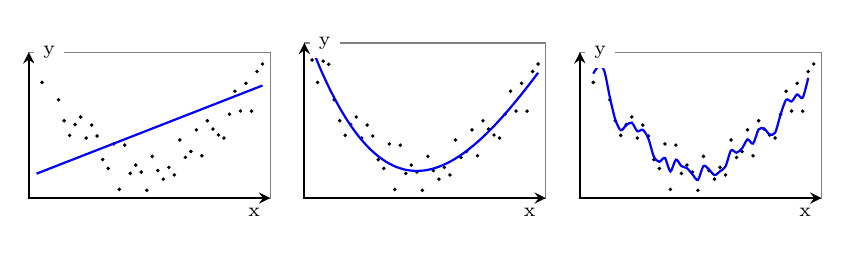
\begin{tikzpicture}[font=\scriptsize,scale=0.70,
				declare function={f(\x)=0.5*pow(abs(\x-2),2)-0.06*pow(\x-2,3);}]
				\foreach \Z in {1,...,42}
				{\pgfmathsetmacro{\X}{\Z/10}
					\pgfmathsetmacro{\Y}{f(\X)+0.9*rnd}
					\ifnum\Z=1
					\xdef\LstOne{(\X,\Y)}
					\xdef\LstTwo{"(\X,\Y)"}
					\else
					\xdef\LstOne{\LstOne (\X,\Y)}
					\xdef\LstTwo{\LstTwo,"(\X,\Y)"}
					\fi}
				\begin{scope}[local bounding box=over,xshift=-5cm]
					\foreach \Z in {1,...,40}
					{\pgfmathsetmacro{\Last}{{\LstTwo}[\Z-1]}
						\pgfmathsetmacro{\Current}{{\LstTwo}[\Z]}
						\pgfmathsetmacro{\Next}{{\LstTwo}[\Z+1]}
						%\typeout{\Last,\Current,\Next}
						\edef\temp{\noexpand\path ($0.6*\Current+0.2*\Last+0.2*\Next$)   coordinate 
							(p\Z);}
						\temp
						\ifnum\Z=1
						\xdef\LstThree{(p\Z)}
						\else
						\xdef\LstThree{\LstThree (p\Z)}
						\fi
					}
					\foreach \Z in {1,...,42}
					{\pgfmathsetmacro{\Coor}{{\LstTwo}[\Z-1]}
						\fill \Coor circle[radius=1pt];
					}
					\draw[thick,blue] plot[smooth] coordinates \LstThree;
				\end{scope}
				%
				\begin{scope}[local bounding box=good,xshift=-10cm]
					\foreach \Z in {1,...,42}
					{\pgfmathsetmacro{\Coor}{{\LstTwo}[\Z-1]}
						\fill \Coor circle[radius=1pt];
					}
					\draw[thick,blue] plot[smooth,domain=0.1:4.2,variable=\x] (\x,{f(\x)+0.45});
				\end{scope}
				%
				\begin{scope}[local bounding box=under,xshift=-15cm]
					\foreach \Z in {1,...,42}
					{\pgfmathsetmacro{\Coor}{{\LstTwo}[\Z-1]}
						\fill \Coor circle[radius=1pt];
					}
					\draw[thick,blue] (0.1,0.4) -- (4.2,2);
				\end{scope}
				%
				\foreach \X in {over,good,under}
				{\draw[gray,thin] ([xshift=-3pt,yshift=3pt]\X.north west) rectangle 
					([xshift=3pt,yshift=-3pt]\X.south east);
					\draw[stealth-stealth,thick] ([xshift=-3pt,yshift=3pt]\X.north west) node[right=1.5pt,fill=white]{y} 
					|- ([xshift=3pt,yshift=-3pt]\X.south east) node[below left]{x};}
			\end{tikzpicture}
			\vspace*{-3mm}
			\captionof{figure}{Models with different complexity for a simple linear regression learning}
			\label{fig:1}
		\end{figure}
	
		From left to right, as the model becomes more complicated, it tends to fit the training data better, i.e., a smaller training loss. But what about their inference performance on unseen data?
	\end{frame}

	\begin{frame}[t]
		\frametitle{A Quick Review on the Classic Bias-variance Trade-off}
		\scriptsize
		\textbf{\small Bias-variance trade-off}\\
		
		\vspace{2mm}
		A good model should have a good \textbf{generalizability}, meaning that it can predict accurately on new data, unseen in training. To study the performance on new data, we typically assume training examples $(\mathbf{x}_i, y_i)$ are sampled randomly from a probability distribution $P$ over $\mathbb{R}^d \times \mathbb{R}$ and test examples are also drawn independently from $P$.\\
		
		\vspace{1mm}
		The challenge comes from the mis-match between the goals of minimizing the empirical risk and minimizing the \textbf{true risk} (or \textbf{test error}) $\mathbb{E}_{(\mathbf{x}, y)\sim P}[L(h(\mathbf{x}), y)]$. Suppose the true model is $g$ and the random noise is $\epsilon$. Recall that the test error can be decomposed into:
		\begin{equation}
			\mathbb{E}_{(\mathbf{x}, y)\sim P}[L(h(\mathbf{x}), y)] = (\mathbb{E}(h(\mathbf{x})) - g(\mathbf{x}))^2 + \text{Var}(h(\mathbf{x})) + \text{Var}(\epsilon)
			\label{eq:1}
		\end{equation}
		
		\vspace{-2mm}
		\begin{figure}[H]
			\centering
			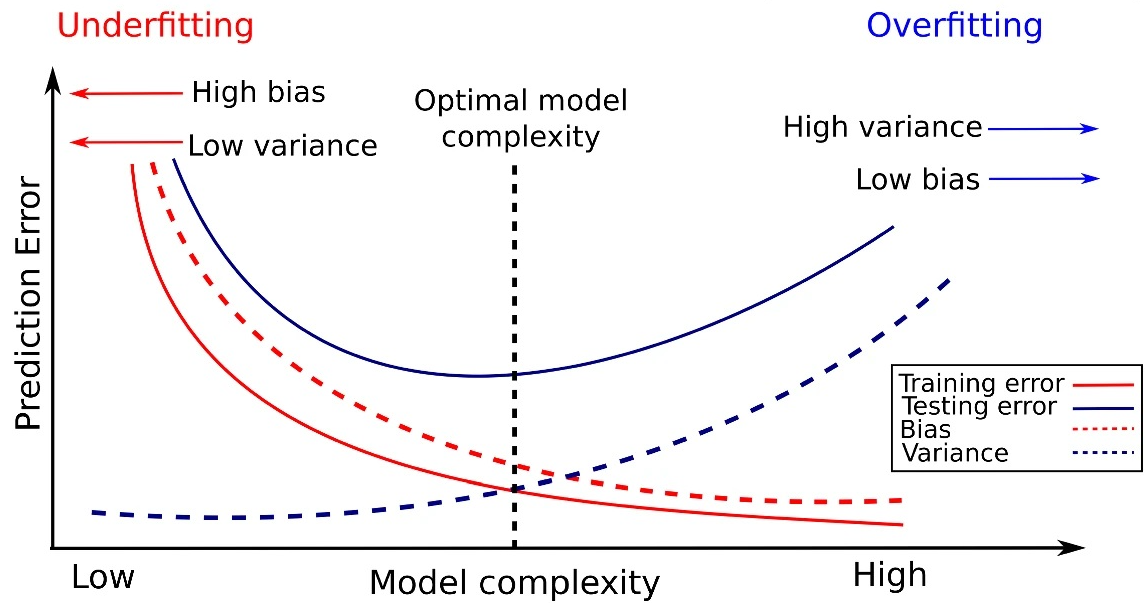
\includegraphics[width=0.6\linewidth]{tradeoff.png}
			\vspace*{-1mm}
			\captionof{figure}{The visualization of bias-variance trade-off (Source: Tharwat, 2019 \cite{tharwat2019parameter})}
			\label{fig:2}
		\end{figure}
	\end{frame}
	
	\section{Part 2. Introduction to Double Descent}
	\begin{frame}[t]
		\frametitle{Introduction to Double Descent}
		\scriptsize
		\textbf{\small Background}\\
		
		\vspace{1mm}
		In modern machine learning, large models, such as deep neural networks and other non-nonlinear models, have become mainstream. These models usually have a huge amount of parameters, and sometimes even more than the number of samples. We call this \textbf{overparameterization}. Despite these models tend to achieve near-zero training loss, it turns out that they can still give very accurate predictions during testing.\\
		
		\vspace{2mm}
		\textbf{\small Double descent}\\
		
		\vspace{1mm}
		Double descent is the phenomenon that: as the model complexity increases, the test risk of trained models first decreases and then increases (the standard U-shape), and then decreases again. The peak in test risk occurs in the “under-parameterized stage” when the models are just barely able to fit the training set. The second descent occurs in the “overparameterized stage” when the model capacity is large enough to \textbf{interpolate} the training data.
		\vspace{-3mm}
		\begin{figure}[H]
			\centering
			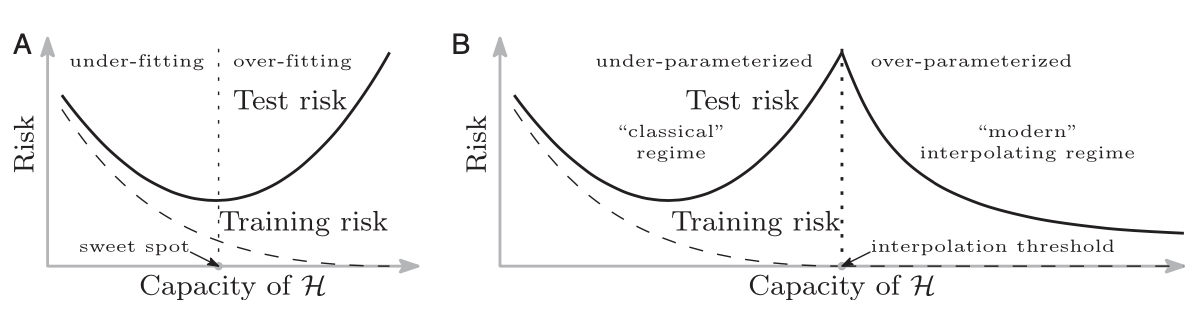
\includegraphics[width=1\linewidth]{double-descent.jpg}
			\vspace*{-5mm}
			\captionof{figure}{The visualization of double descent (Source: Belkin et al., 2019 \cite{belkin2019reconciling})}
			\label{fig:3}
		\end{figure}
	\end{frame}

	\begin{frame}[t]
		\frametitle{Introduction to Double Descent}
		\scriptsize
		\textbf{\small Why does double descent happen?}\\
		
		\vspace{1mm}
		Intuitively, ...
		\begin{itemize}
			\justifying
			\item Belkin et al., 2019 \cite{belkin2019reconciling}\\
			They believe that, the capacity of the function class does not necessarily reflect how well the predictor matches the inductive bias for the problem at hand. Here, the inductive bias that seems appropriate is the \textbf{regularity} or \textbf{smoothness} of a function, which can be measured by a certain function space norm (we don't know, but it exists). By considering larger function classes containing more compatible candidate models, we are able to find interpolating functions that have smaller norm. Thus, increasing function class capacity improves performance of models.\\
			
			\item Nakkiran et al., 2021 \cite{nakkiran2021deep}\\
			They define a new complexity measure called the \textbf{effective model complexity} and conjecture a generalized double descent with respect to this measure.
		\end{itemize}
	
		Alternative explanations proposed by some physicists, ...
		\begin{itemize}
			\justifying
			\item Baldassi et al. (2021) \cite{baldassi2021unveiling} \& Canatar et al. (2021) \cite{canatar2021spectral} \\
			They use methods in statistical physics to investigate the occurrence of double descents in DNN learning. Baldassi et al. posit that the structure of solution space is changed before and after the interpolation threshold. Canatar et al. argue that there could be multiple descents and the model is learning different patterns with different sets of features in each stage. Fundamentally, the switch between these stages is analogous to the \textbf{phase transition} in physics.
		\end{itemize}
		\vspace{1mm}
	\end{frame}
	
	\section{Part 3. A Simple Experiment to See Double Descent}
	\begin{frame}[t]
		\frametitle{A Simple Experiment to See Double Descent}
		\scriptsize
		\textbf{\small Experiment setup}
		\begin{itemize}
			\justifying
			\item Ground-truth distribution $P$ is $(\mathbf{x}, y) \in \mathbb{R}^d \times \mathbb{R}$ with covariates $\mathbf{x} \sim \mathcal{N}(0, I_d)$ and response $y=\mathbf{x}^\intercal \beta + \epsilon$ where the noise term $\epsilon \in \mathcal{N}(0, \sigma^2)$.
			\item We are given $n$ samples $(\mathbf{x_i},y_i)$ from the distribution $P$, and we want to learn a linear model $h_n = \mathbf{x}^\intercal \hat{\beta}$ for estimating $y$ given $x$, which can minimize the test error $R(\hat{\beta})$. Since the features $\mathbf{x}$ is \textbf{isotropic}, the test error can be expressed as:
			\begin{equation}
				R(\hat{\beta}) = \mathbb{E}_{(\mathbf{x}, y)\sim P}[(\mathbf{x}^\intercal \hat{\beta} - y)^2] = ||\hat{\beta} - \beta||^2 + \sigma^2
				\label{eq:2}
			\end{equation}
			\item To train this model, we will start by zero-initialization and run full-batch graident descent on following learning objective:
			\begin{equation}
				 \min_{\hat{\beta}} \frac{1}{n}||\mathbf{X}\hat{\beta} - \mathbf{y}||^2
				 \label{eq:3}
			\end{equation}
			The solution found by gradient descent is $\hat{\beta} = \mathbf{X}^\dagger \mathbf{y}$, where $\mathbf{X}^\dagger$ denotes the pseudoinverse.  $\mathbf{X}^\dagger$ has different values depending on the ratio $n/d$. When $n \geq d$, we are in the “underparameterized” regime and there is a unique minimizer of the objective in Equation (\ref{eq:3}). When $n < d$, we are “overparameterized” and there are many minimizers of Equation (\ref{eq:3}). In this regime, gradient descent finds the minimum with smallest $\mathcal{L}_2$ norm $||\beta||^2$. That is, the solution can be written as:
			\begin{equation}
				\hat{\beta} = \mathbf{X}^\dagger \mathbf{y} = \left\{
				\begin{aligned}
					& \arg\min_{\hat{\beta}}||\hat{\beta}||^2 \  \text{s.t.} \ \mathbf{X}\hat{\hat{\beta}} = \mathbf{y} & \text{when} \ n < d\\
					& \arg\min_{\hat{\beta}}||\mathbf{X}\hat{\beta} - \mathbf{y}||^2 & \text{when} \ n \geq d
				\end{aligned}
				\right.
				\label{eq:4}
			\end{equation}
		\end{itemize}
	\end{frame}

	\begin{frame}[t]
		\frametitle{A Simple Experiment to See Double Descent}
		\scriptsize
		\textbf{\small Analytical results}
		
		\vspace{1mm}
		According to Nakkiran (2019) \cite{nakkiran2019more} and Hastie et al. (2022) \cite{hastie2022surprises}, let's denote the ratio of $n/d$ as $\gamma$, and the test error in underparameterized and overparameterized regime can be expressed as:
		\begin{equation}
			R(\gamma) = \left\{
			\begin{aligned}
				& \sigma^2\frac{\gamma}{1-\gamma} & \text{when} \ \gamma < 1\\
				& r^2(1-\frac{1}{\gamma}) + \sigma^2\frac{1}{1-\gamma} & \text{when} \ \gamma > 1
			\end{aligned}
			\right.
			\label{eq:5}
		\end{equation}
		
		\textbf{\small Results on synthetic data}
		\begin{figure}[H]
			\centering
			\subfloat
			{{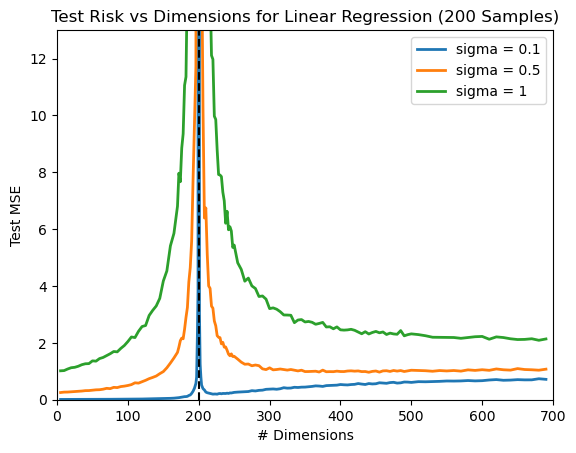
\includegraphics[width=5.5cm]{experiment_1.png} }}%
			\qquad
			\subfloat
			{{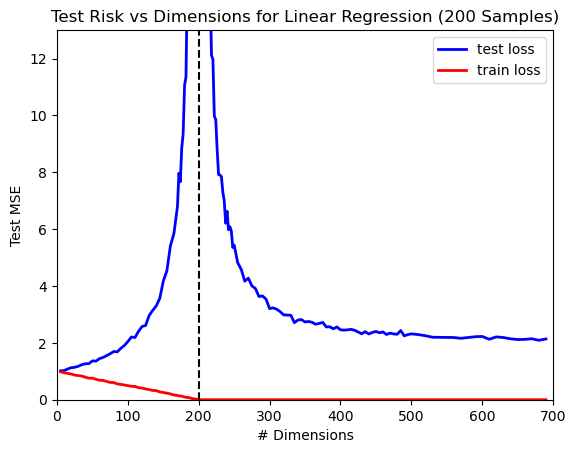
\includegraphics[width=5.5cm]{experiment_2.png} }}%
			\label{fig:4}
		\end{figure}
	\end{frame}

	\section{Part 4. Why Does This Matter?}
	\begin{frame}[t]
		\frametitle{Why Does This Matter?}
		\scriptsize
		Since we have seen that double descent can take place even on linear regression learning tasks, it shouldn't be a big surprise to reproduce it in more complicated models such as DNN, kernel machines, and transformers. Now the question is: why does this matter? \\
		
		\vspace{1mm}
		\begin{itemize}
			\justifying
			\item Theoratically justify the development of complicated models, as it suggests that increasing model complexity may not always be detrimental, and there can be a regime where larger models can perform better.
			\item Double descent has spurred research into understanding the theoretical underpinnings of this phenomenon. It has led to new insights into the geometry of high-dimensional spaces and the optimization landscape of overparameterized models.
		\end{itemize}
	
		\begin{figure}[H]
			\centering
			\subfloat
			{{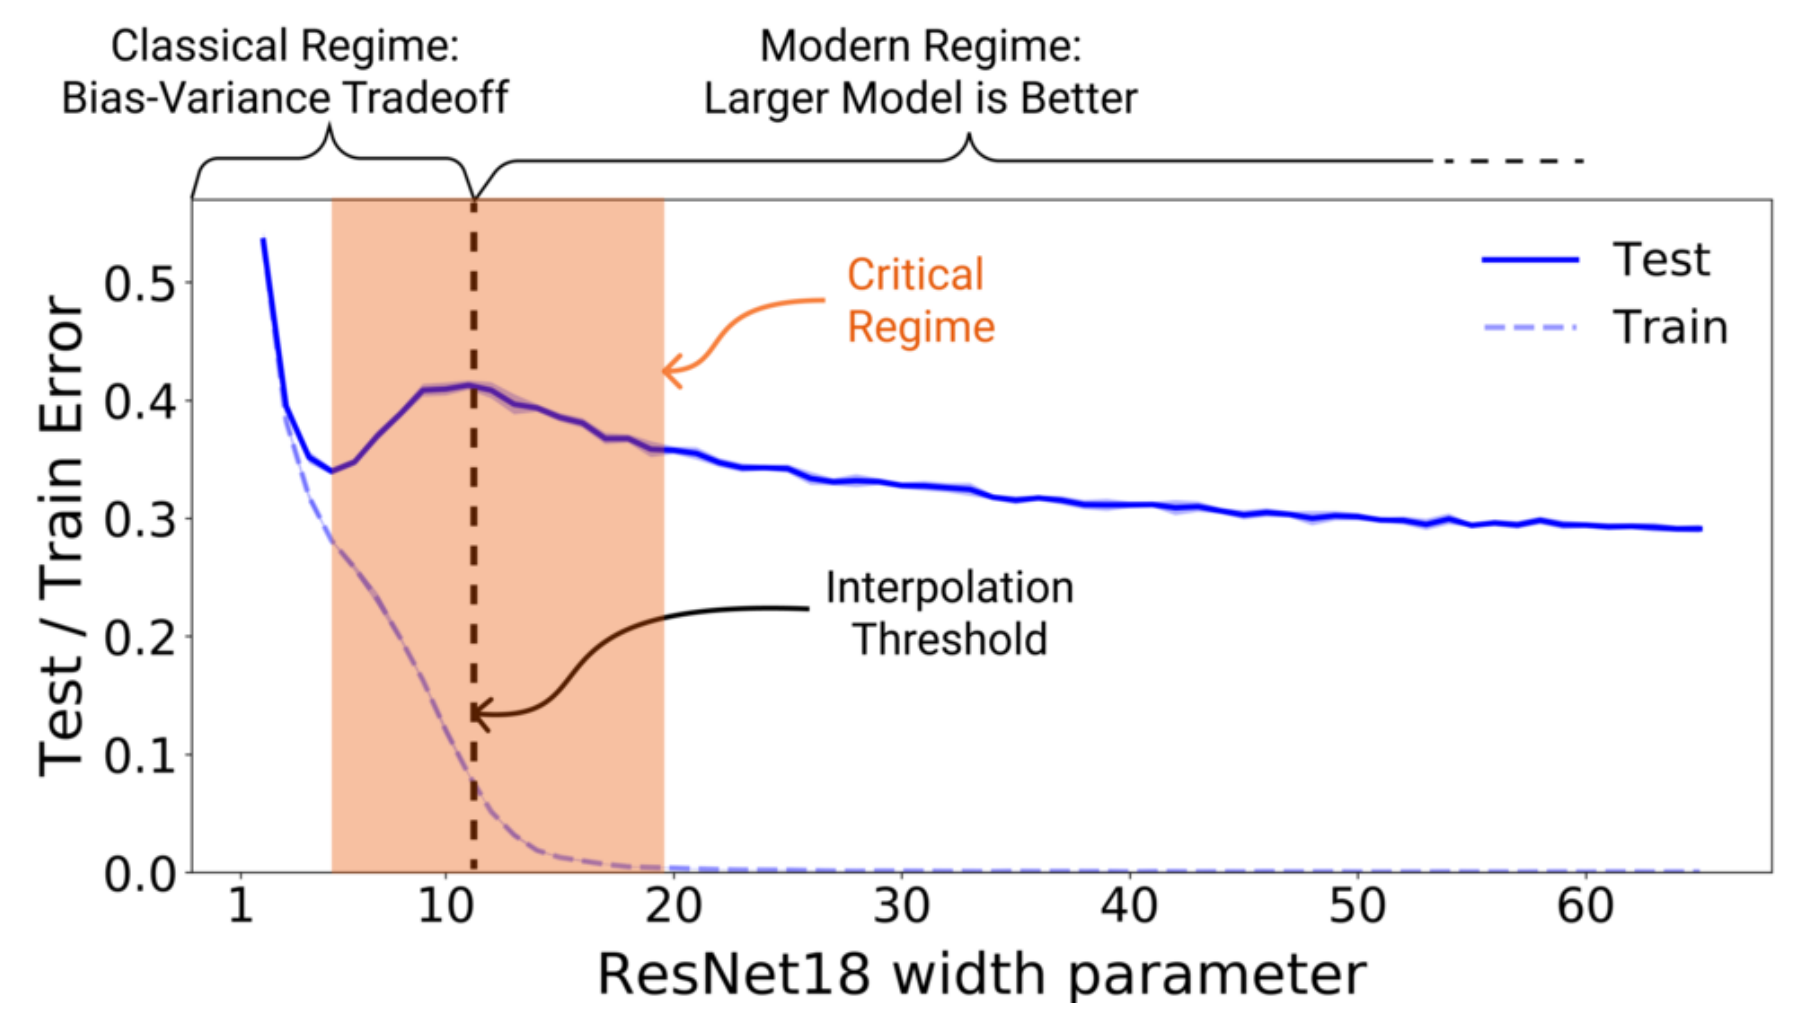
\includegraphics[width=5.5cm]{resnet_dd.png} }}%
			\qquad
			\subfloat
			{{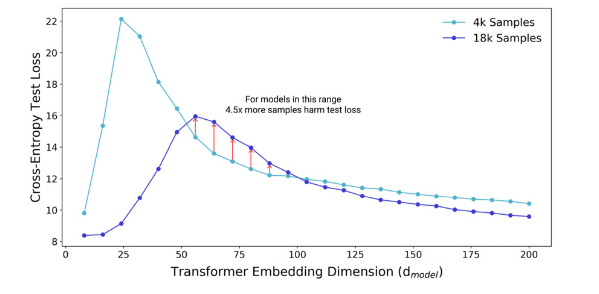
\includegraphics[width=5.5cm]{transfomer_dd.jpg} }}%
			\captionof{figure}{Double descent on ResNet and Transformer (Source: Nakkiran et al. (2021) \cite{nakkiran2021deep})}
			\label{fig:5}
		\end{figure}
	\end{frame}
	
	\section{Part 5. Plan for the Next}
	\begin{frame}[t]
		\frametitle{Part 5. Plan for the Next}
		\scriptsize
		\textbf{\small Investigate model pruning technique in a wider landscape}\\
		
		\vspace{1mm}
		Model pruning in neural networks involves removing certain connections or parameters from the network to make it smaller and more computationally efficient. Despite the reduction in size, effective pruning methods aim to retain or even improve the model's performance by preserving critical connections.
		\vspace{-3mm}
		\begin{figure}[H]
			\centering
			\subfloat
			{{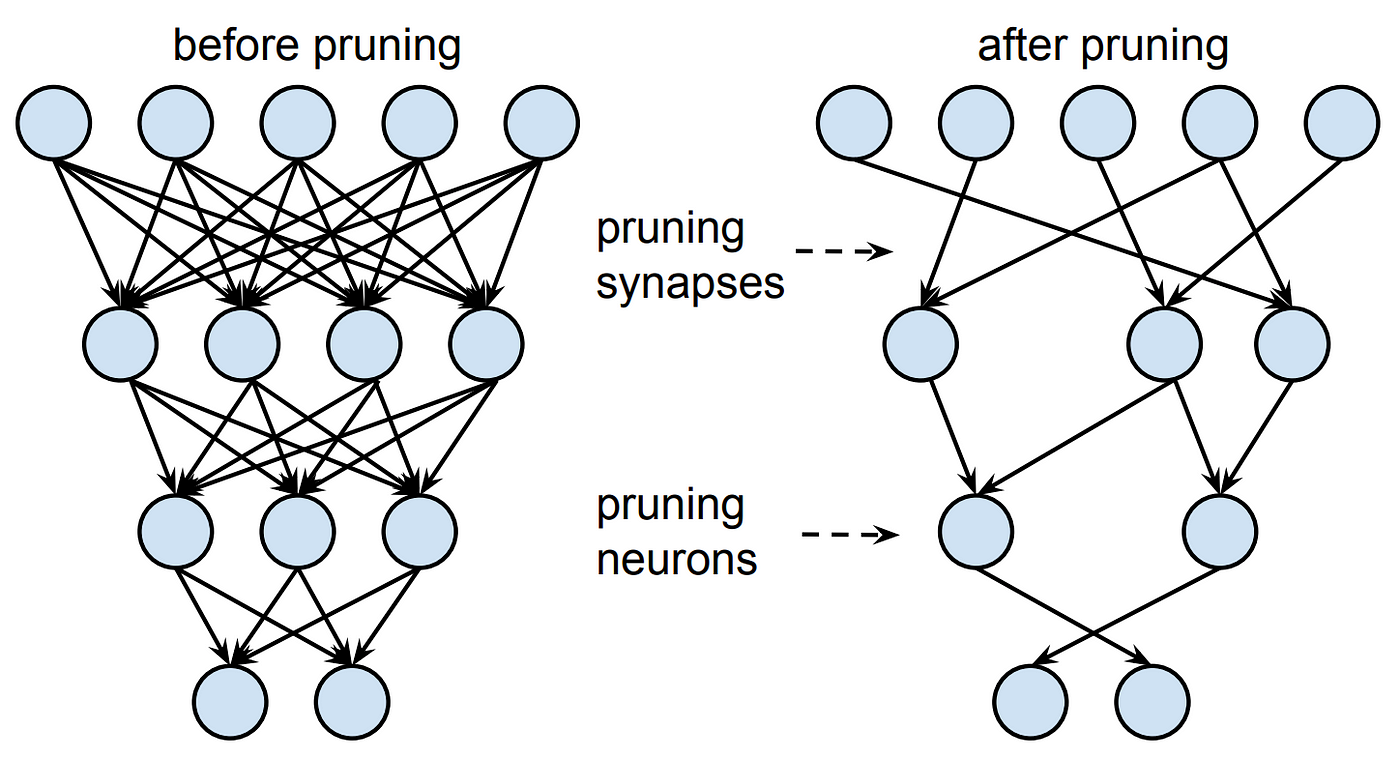
\includegraphics[width=5cm]{pruning.png} }}%
			\qquad
			\subfloat
			{{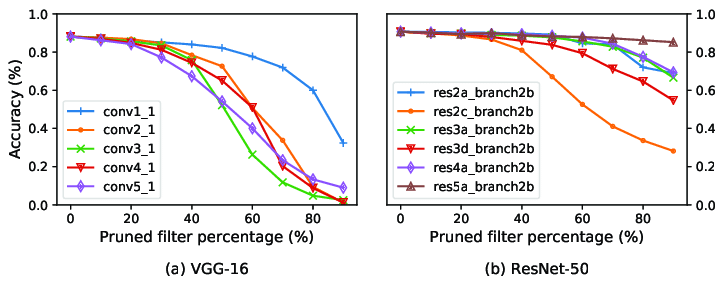
\includegraphics[width=6cm]{pruned_accs.png} }}%
			\label{fig:6}
		\end{figure}
	
		\textbf{\small Build a better classifier for P300 brain-computer interface}
		
		\vspace{-3mm}
		\begin{figure}[H]
			\centering
			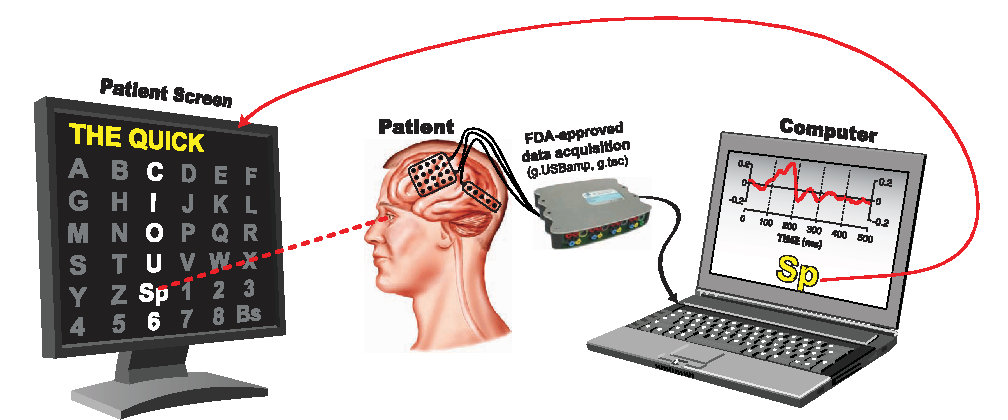
\includegraphics[width=0.55\linewidth]{p300_speller.png}
			\vspace*{-3mm}
			\label{fig:p300}
		\end{figure}
	\end{frame}
	
	\section{Part 6. References}
	\begin{frame}[t]
		\frametitle{References}
		\tiny
		\bibliographystyle{plain}
		\bibliography{refs}
		
	\end{frame}
		
	
\end{document}